% 第三章

\chapter{移植PKE的总体设计}

\section{移植PKE到K210的背景}

接下来,本文将通过阐述PKE移植前的开发环境与移植后的预期收益,
介绍移植PKE到K210的背景。

\subsection{PKE移植前开发环境介绍}

PKE移植前的运行环境主要分为两种,分别是硬件环境和模拟器环境。
他们的总体情况是一致的,但还是有一些细微的区别。

在模拟器环境上,PKE运行在spike模拟的RISC-V 64位机器上。
而spike模拟器则运行在宿主机Ubuntu上。
当PKE需要使用外部设备的I/O功能时,
PKE就通过调用spike提供的HTIF接口,
让Ubuntu提供I/O功能,以访问宿主机上的外设资源。

如下图,本文给出了模拟器环境的系统架构。

\begin{figure}[htbp]
    \vspace{13pt} % 调整图片与上文的垂直距离
    \centering
    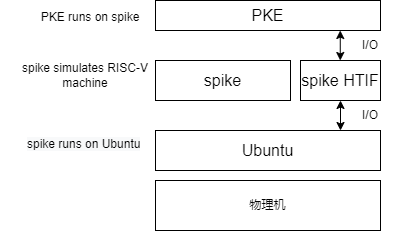
\includegraphics[width=0.6\textwidth]{images/spike_structure.png}
    \caption{模拟器环境架构}\label{模拟器环境架构} % label 用来在文中索引
\end{figure}

在硬件环境上,我们的系统是运行上PYNQ-Z2开发板上。
PYNQ-Z2开发板是Xilinx公司的一款开发板,
它具有丰富的外设资源、强大的性能。此外,它还兼容了Arduino和树莓派接口。

PYNQ-Z2搭载了FPGA系统和ARM处理器。FPGA可以烧录RISC-V CPU软核,
ARM硬核可以运行Ubuntu操作系统。我们的代理内核PKE运行在RISC-V CPU软核上,
而提供外设功能的Ubuntu则运行在ARM硬核上。
PKE和Ubuntu之间是通过riscv-fesvr通信的。
riscv-fesvr是PYNQ开发板上的重要工具,没有它,PKE就无法调用ARM上的Ubuntu I/O接口。
riscv-fesvr通过共享内存的方式,接收PKE的请求,使用ARM端的资源,并向PKE提供资源与功能。

如下图,本文给出了硬件环境的系统架构。

\begin{figure}[htbp]
    \vspace{13pt} % 调整图片与上文的垂直距离
    \centering
    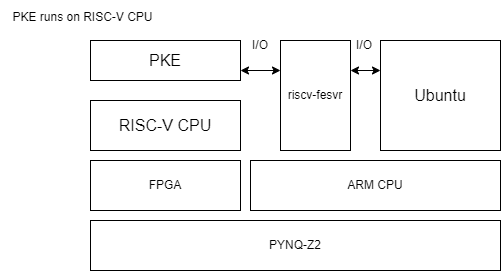
\includegraphics[width=0.6\textwidth]{images/pke_hardware_env.drawio.png}
    \caption{硬件环境架构}\label{硬件环境架构} % label 用来在文中索引
\end{figure}

\subsection{PKE移植后的预期收益}

\section{移植PKE的目标}

\begin{enumerate}
    \item 用户态程序无感知
    \item 减少实验操作者对移植的感知
    \item 降低PKE在物理环境开发的成本
    \item 提高实验操作者的开发效率
    \item 降低PKE后续移植的成本
\end{enumerate}

\section{移植PKE的需求分析}

\section{移植K210前PKE的总体设计}

\subsection{系统架构}

\subsection{主要功能模块介绍}

\subsection{执行流程}

\section{移植PKE到K210的技术方案}

\section{移植K210后PKE的总体设计}

\subsection{系统架构}

\subsection{主要功能模块介绍}

\subsection{执行流程}
